\chapter{Results}
\index{Results@\emph{Results}}%

\section{Quantity Oppositions in Ictus position}


Ternary quantity contrast is only in primary stressed syllables. To analyze vowel duration measurements in all three quantities, a subset of only primary stressed syllables is taken from the dataset. 
At the song level, the kalevala meter avoids short stressed syllables (Q1) in ictus position, preferring Q2 or Q3 (long and overlong) syllables to fall on the beat. In off-ictus postion, short stressed (Q1) syllables are preferred while Q3 avoided.


\begin{figure}[htb]
\centering
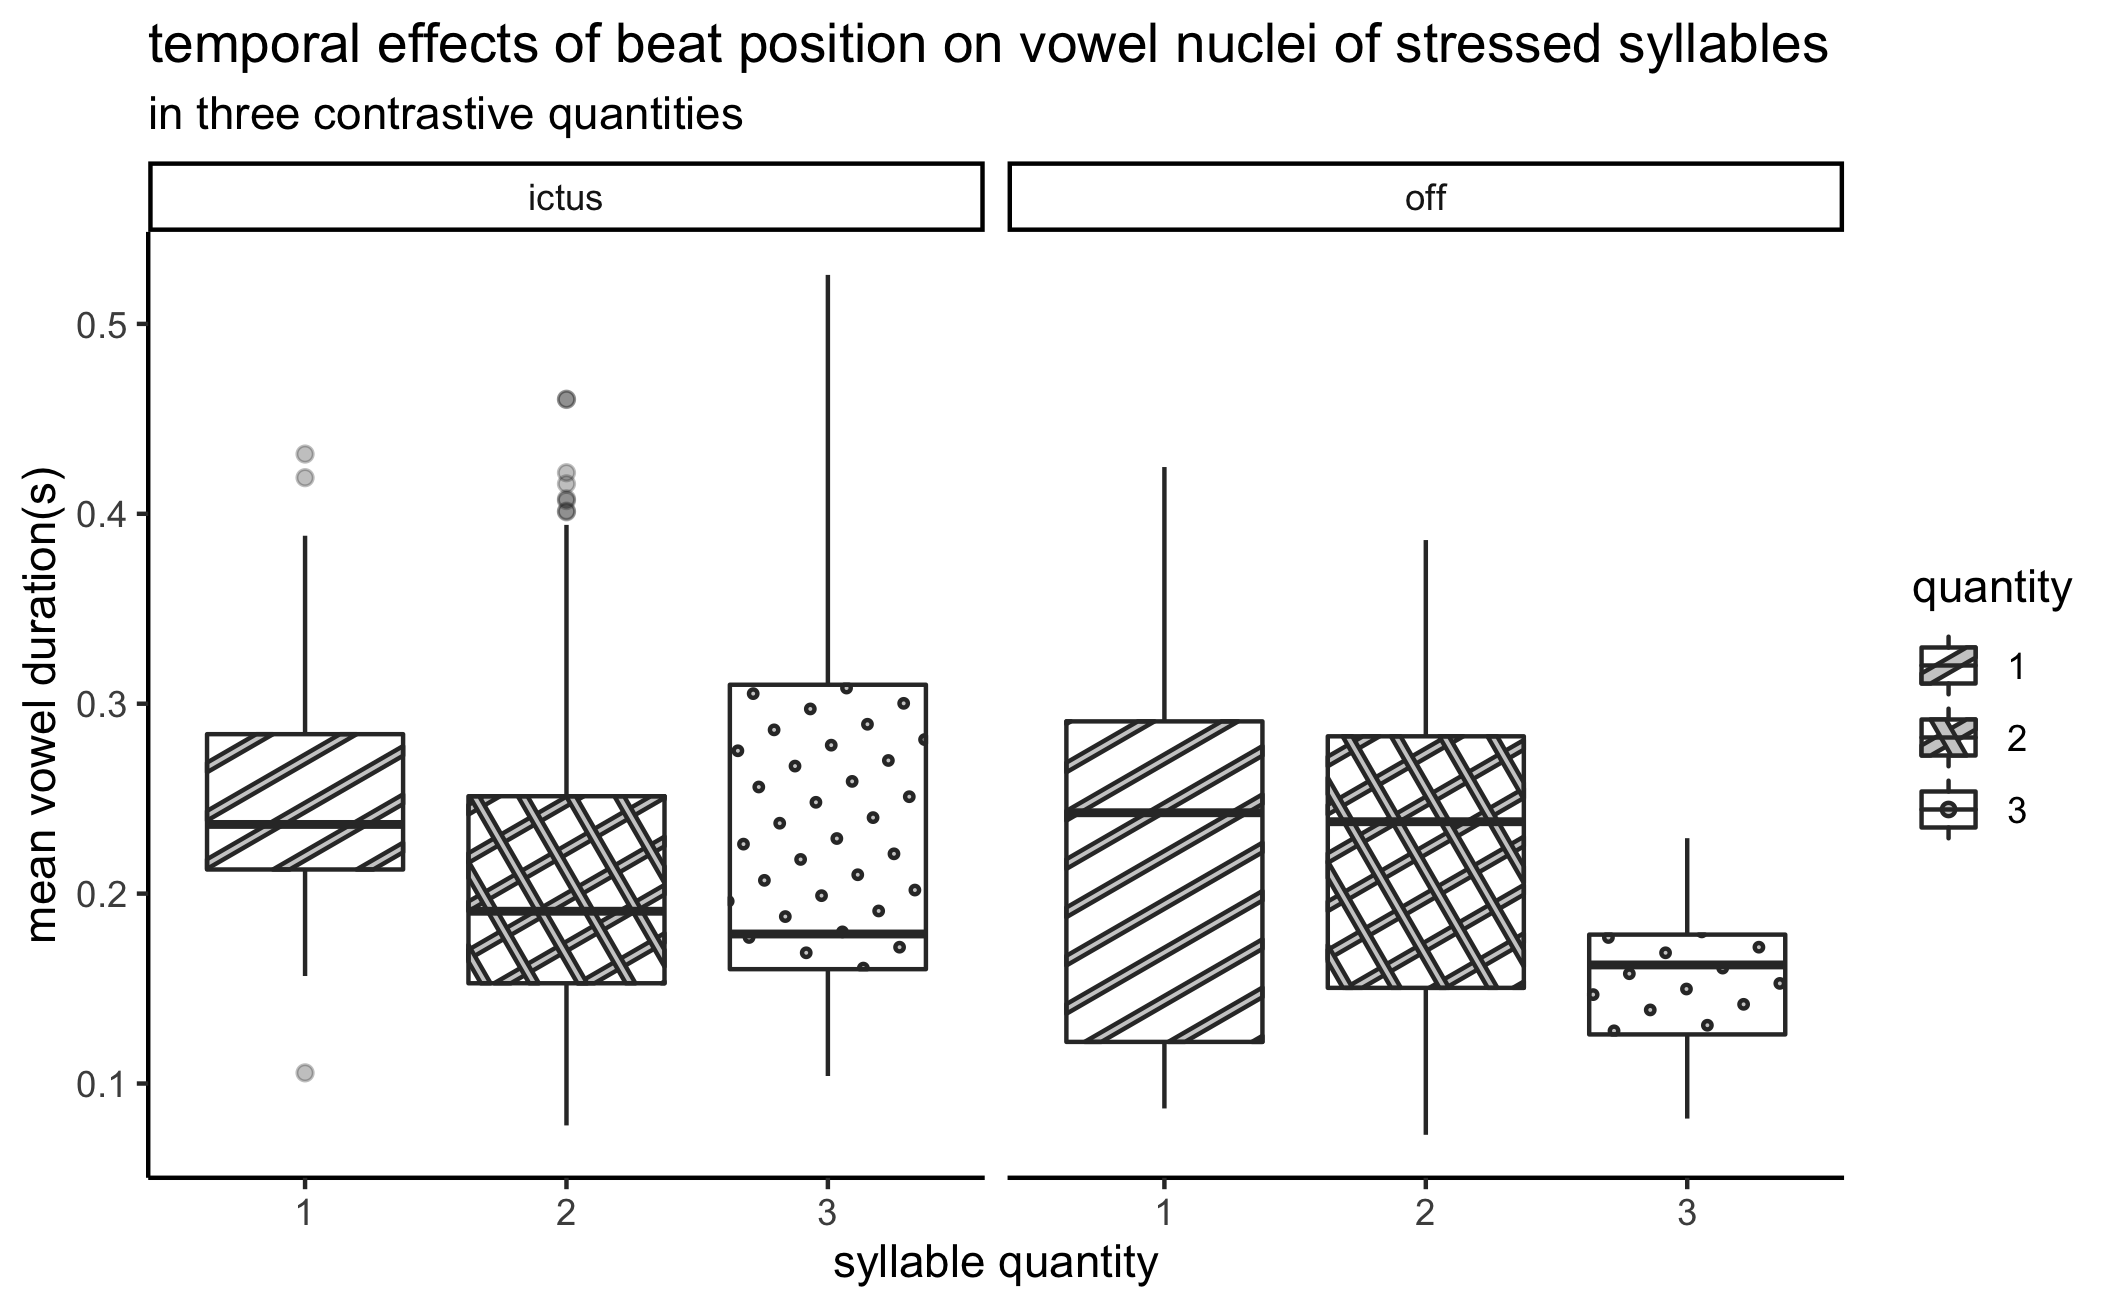
\includegraphics[width =\textwidth]{/Users/sarah/Git/regilaul_project/manuscript/results/q_dur.png}
\caption{density plot of vowel durations in three syllable quantities}
\label{qdur}

\end{figure}
%\begin{wrapfigure}{l}{\textwidth}
%\centering
%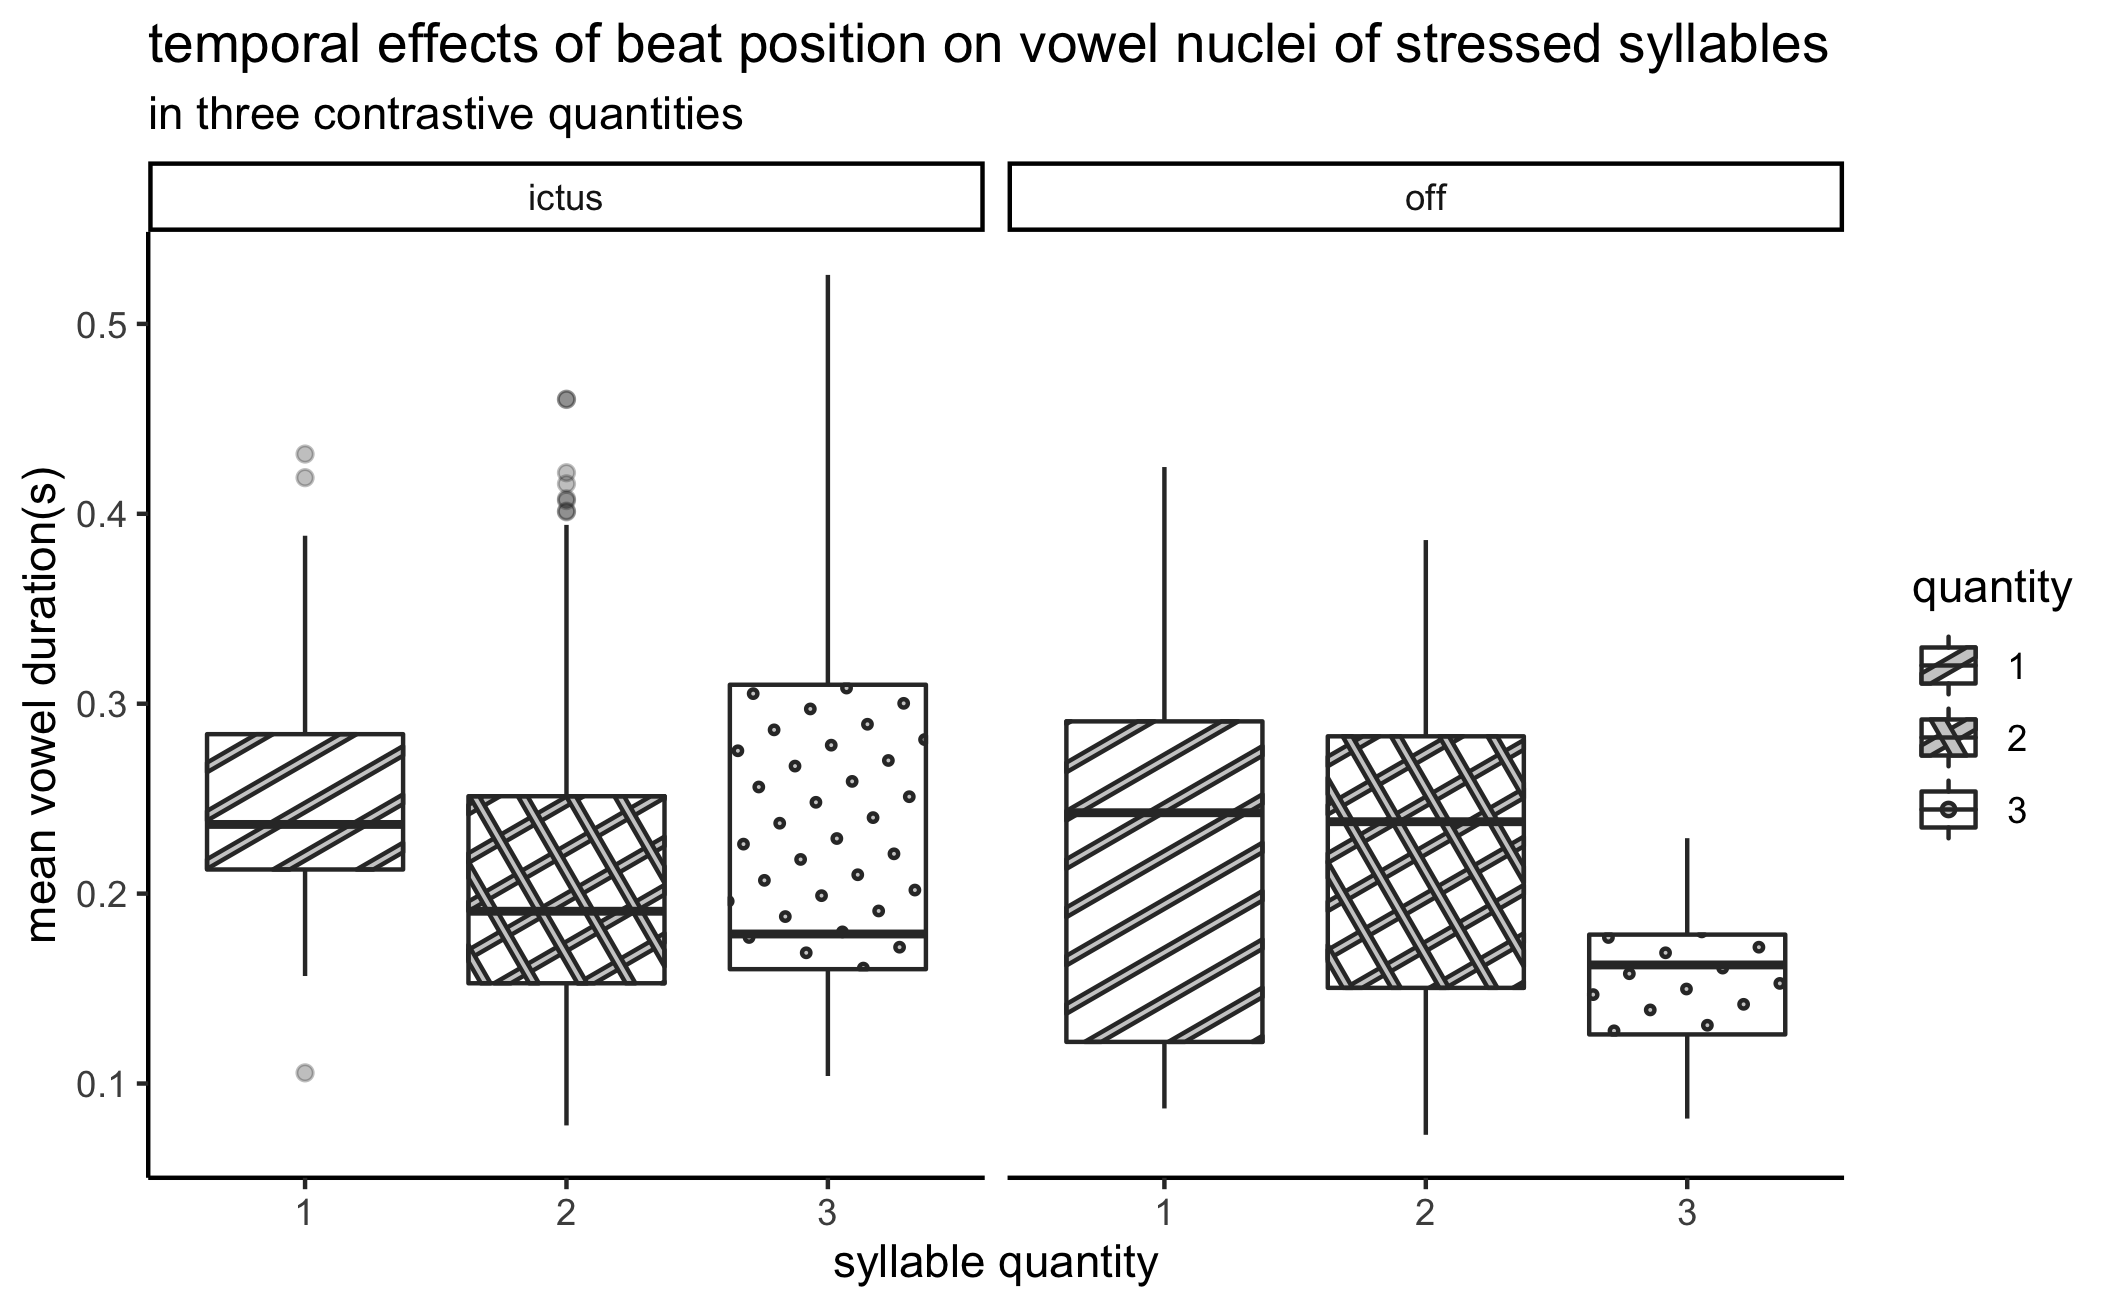
\includegraphics[width =\textwidth]{/Users/sarah/Git/regilaul_project/manuscript/results/q_dur.png}
%\caption{density plot of vowel durations in three syllable quantities}
%\label{qdur}
%
%\end{wrapfigure}


\ref{qdur} shows the vowel durations of all three syllable quantities, grouped by ictus and off-ictus positions in the song. In ictus position, median vowel duration descends as quantity increases, with the greatest difference between Q1 and Q2. Off the beat, a similar descending pattern is evident: however, in this case the largest difference is between Q2 and Q3 syllables. 
 The intercept is set at ictus position, Q1. Findings are significant results for Q2(p<0.001), Q3, and off-ictus positions (p< 0.05). Comparison with null model was statistically significant (p<0.001). For full model output see \ref{qdurfixed} and \ref{qdurrandoms} in Appendix A. In context of earlier findings that the quantity contrast was ``lost" at the syllable level, the decrease in vowel duration as syllable weight increases supports the notion that the contrast is preserved at the segmental level. That is, rather than the full syllable lengthening in duration, the song-level isochrony of syllable-notes results in vowel nuclei shortening to accommodate codas in Q2, and further for geminates and complex codas in Q3. 
 
 
A null model constructed containing only random effects was compared to the design model by two-way ANOVA. Results are significant for the design model (p < 0.001***), and so I reject the null hypothesis. 

These data and analysis support both syllable quantity and ictus as predictors for vowel duration. 



%\begin{equation}
%$$lmer(duration ~ quantity + ictus + quantity * ictus + (1 | song) + (1 | word) + (1 | performer))$$ \\
%
%$$lmer(duration ~ (1 | song) + (1 | word) + (1 | performer))$$
%
%
%
%\end{equation}
\section{stress and unstress}


\subsection{duration}

\begin{figure}[htbp]
\centering
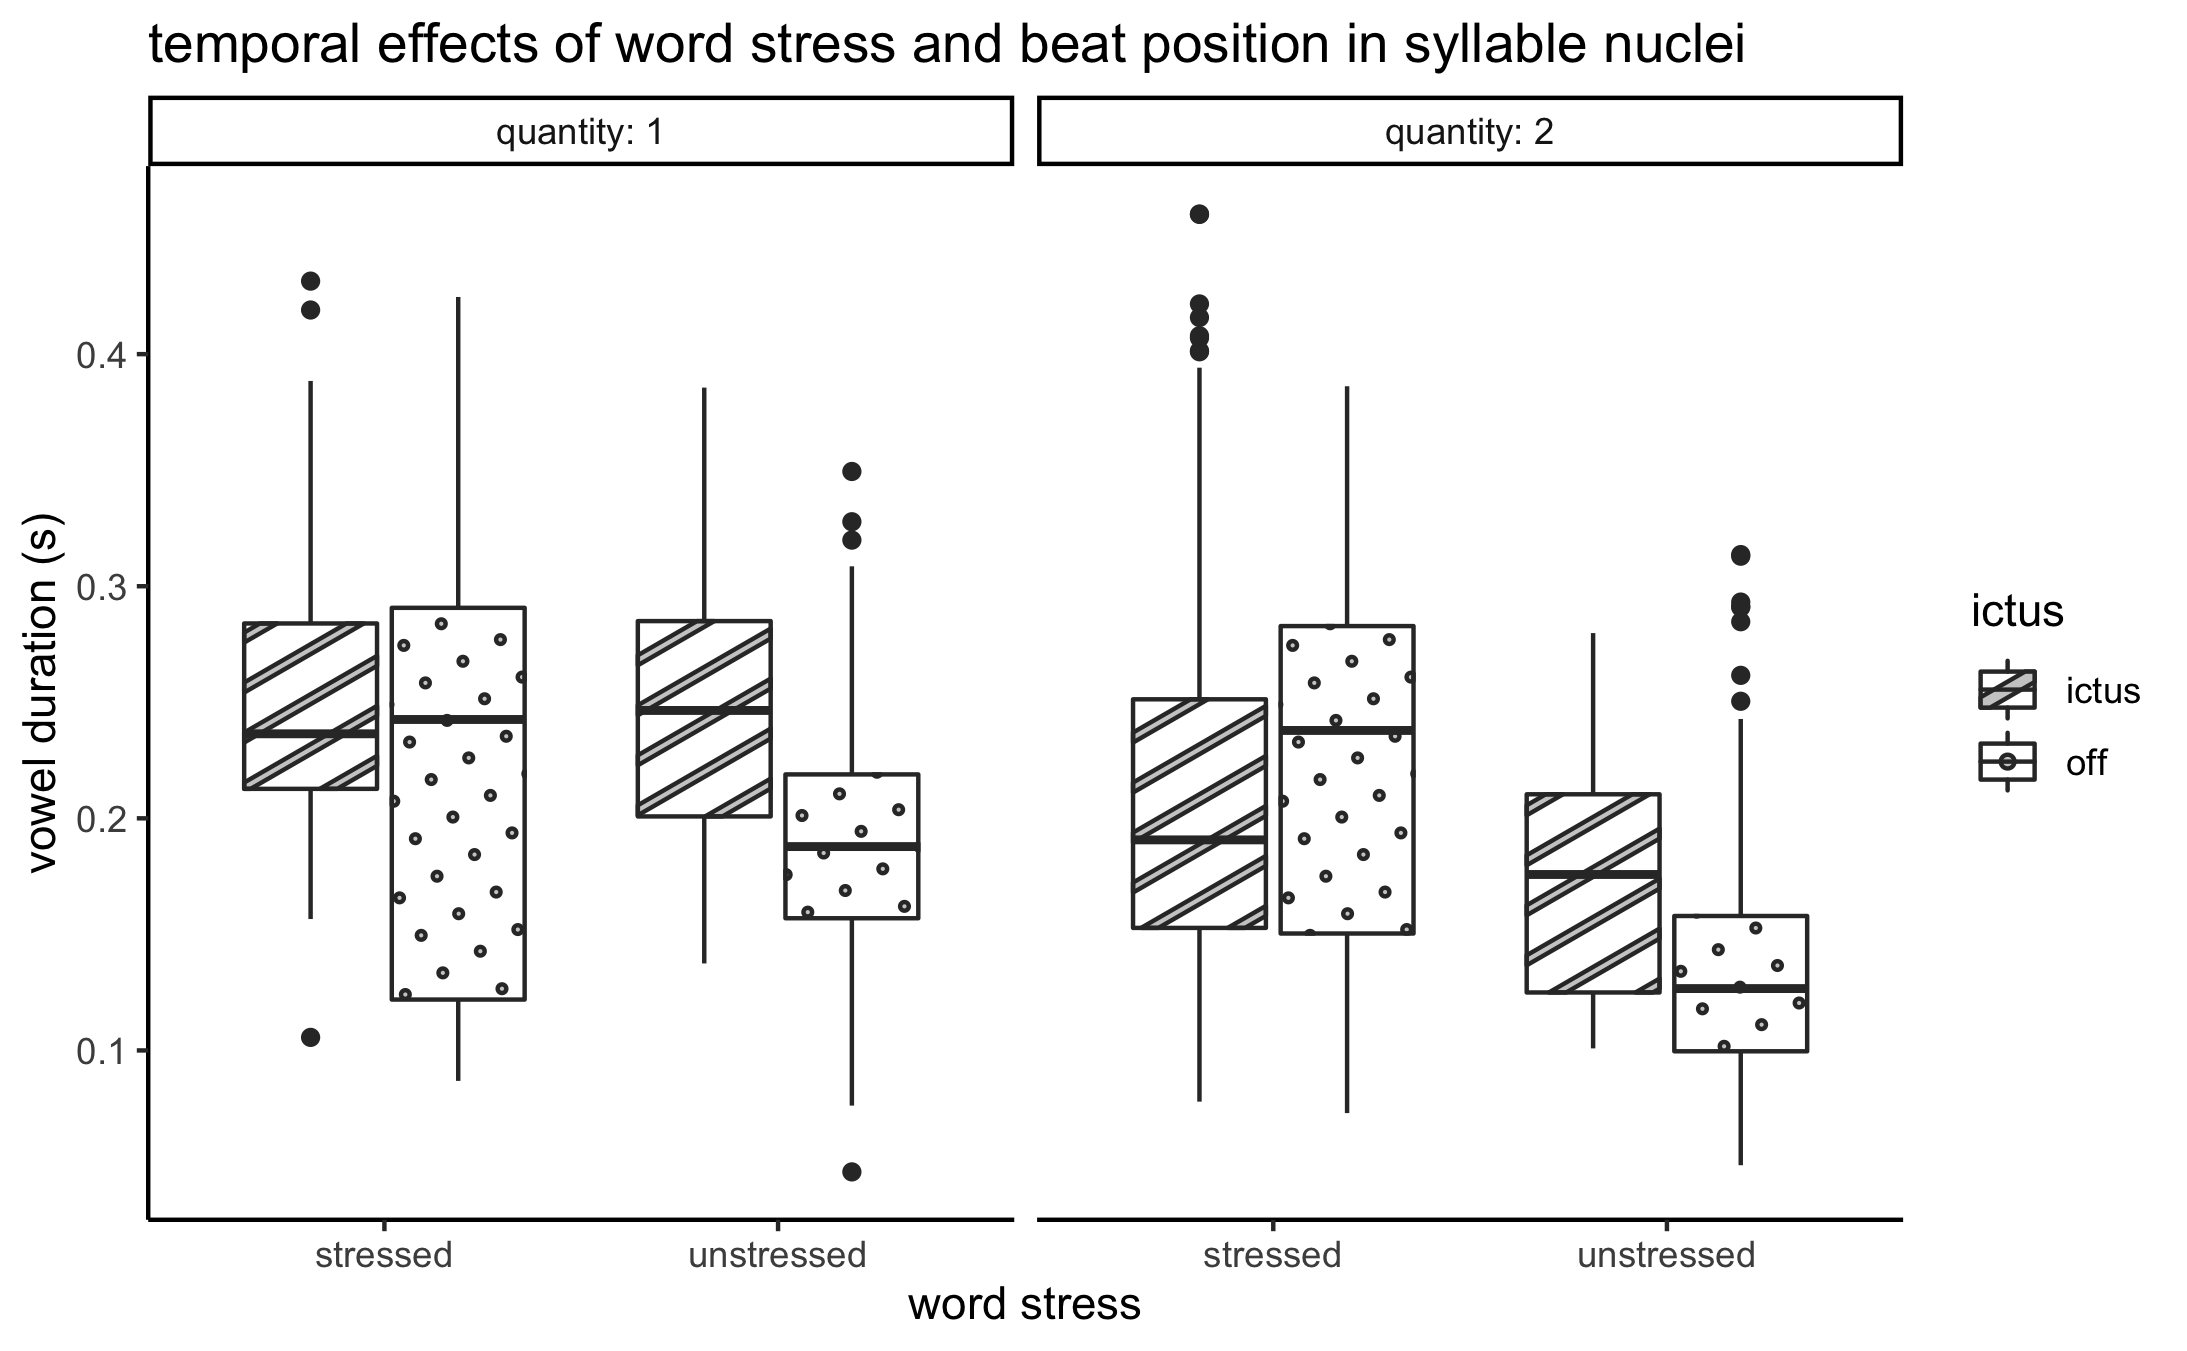
\includegraphics[width = \textwidth]{/Users/sarah/Git/regilaul_project/manuscript/results/dur_density_qfac.png}
\caption{vowel durations of stressed and unstressed Q1 and Q2 syllables falling on (ictus) and off the beat}
\label{durstrick}
\end{figure}

The two graphs in \ref{durstrick} illustrate the distribution of vowel durations in stressed and unstressed syllables falling on and off the beat. In Q1 syllables, ictus position predicts longer vowels in both stressed and unstressed syllables, while stressed syllables are longer overall than unstressed. In Q2, we see longer vowel durations for ictus position in stressed syllables, and higher means for ictus position in unstressed, though the distributions overlap much more here. \\

Linear mixed-effects model results are significant for off-ictus (p<0.05**), stressed (p<0.001***), and Q2 (p<0.001***). 

\begin{figure}[htpb]
\centering
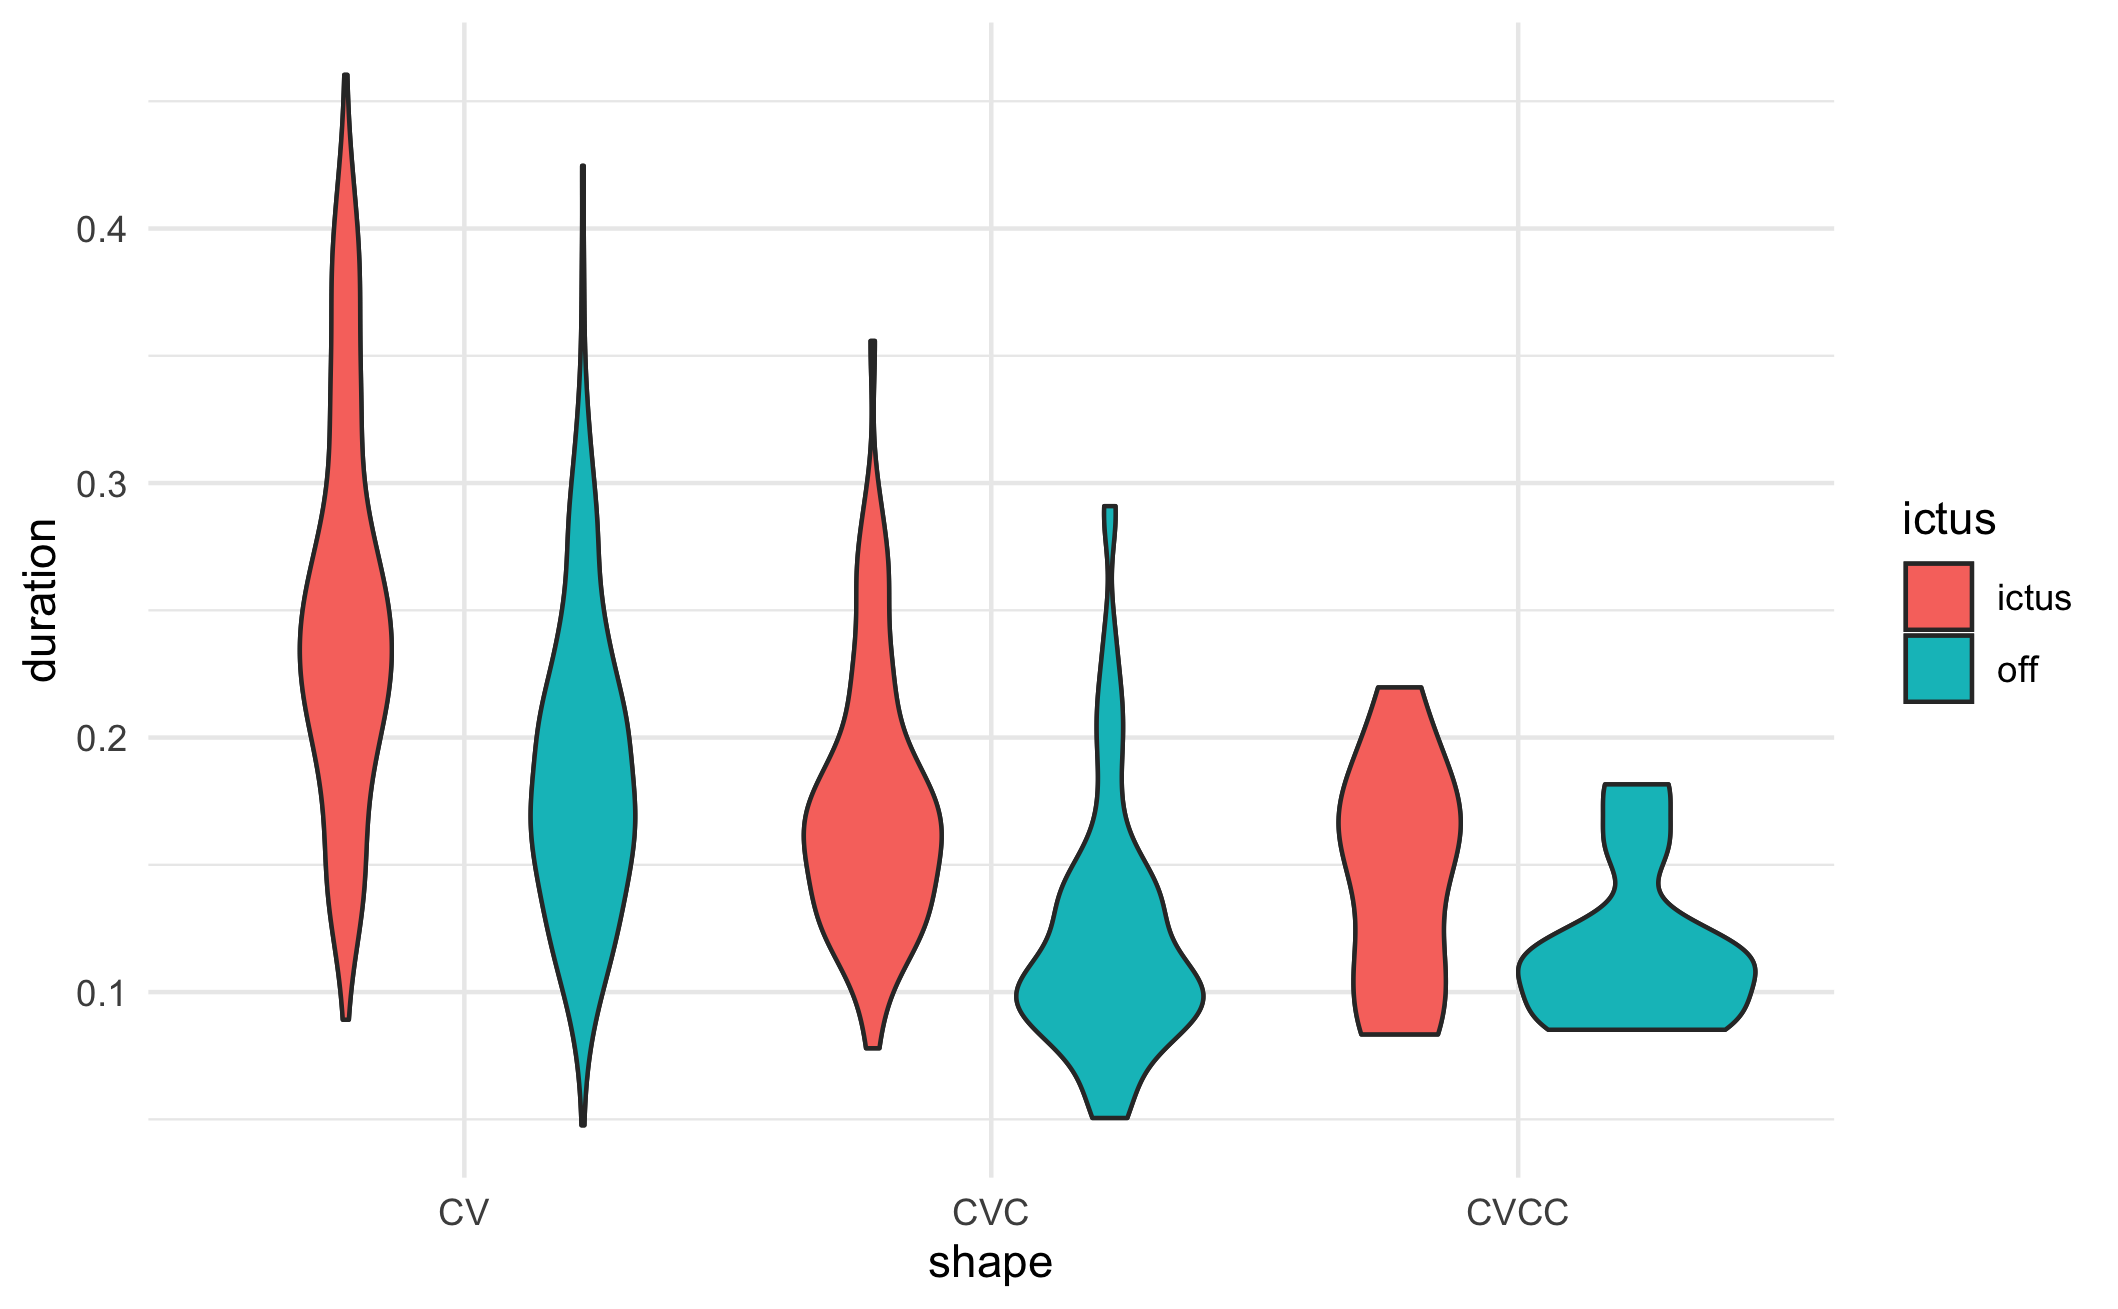
\includegraphics[width=\textwidth]{/Users/sarah/Git/regilaul_project/manuscript/results/dur_shape_ictus.png}
\caption{vowel dur(s) by beat position and syll. shape}
\label{ickdursh}
\end{figure}

Compared to Q1 unstressed syllables in ictus position (the intercept,  off-ictus positions have a negative slope and are overall shorter. Stressed syllables have a small positive slope, indicating longer vowel durations. Q2 syllables have a negative slope, highlighting the shortening of syllable nuclei to accomodate the codas of these syllables. 


\begin{figure}[htbp]
\centering
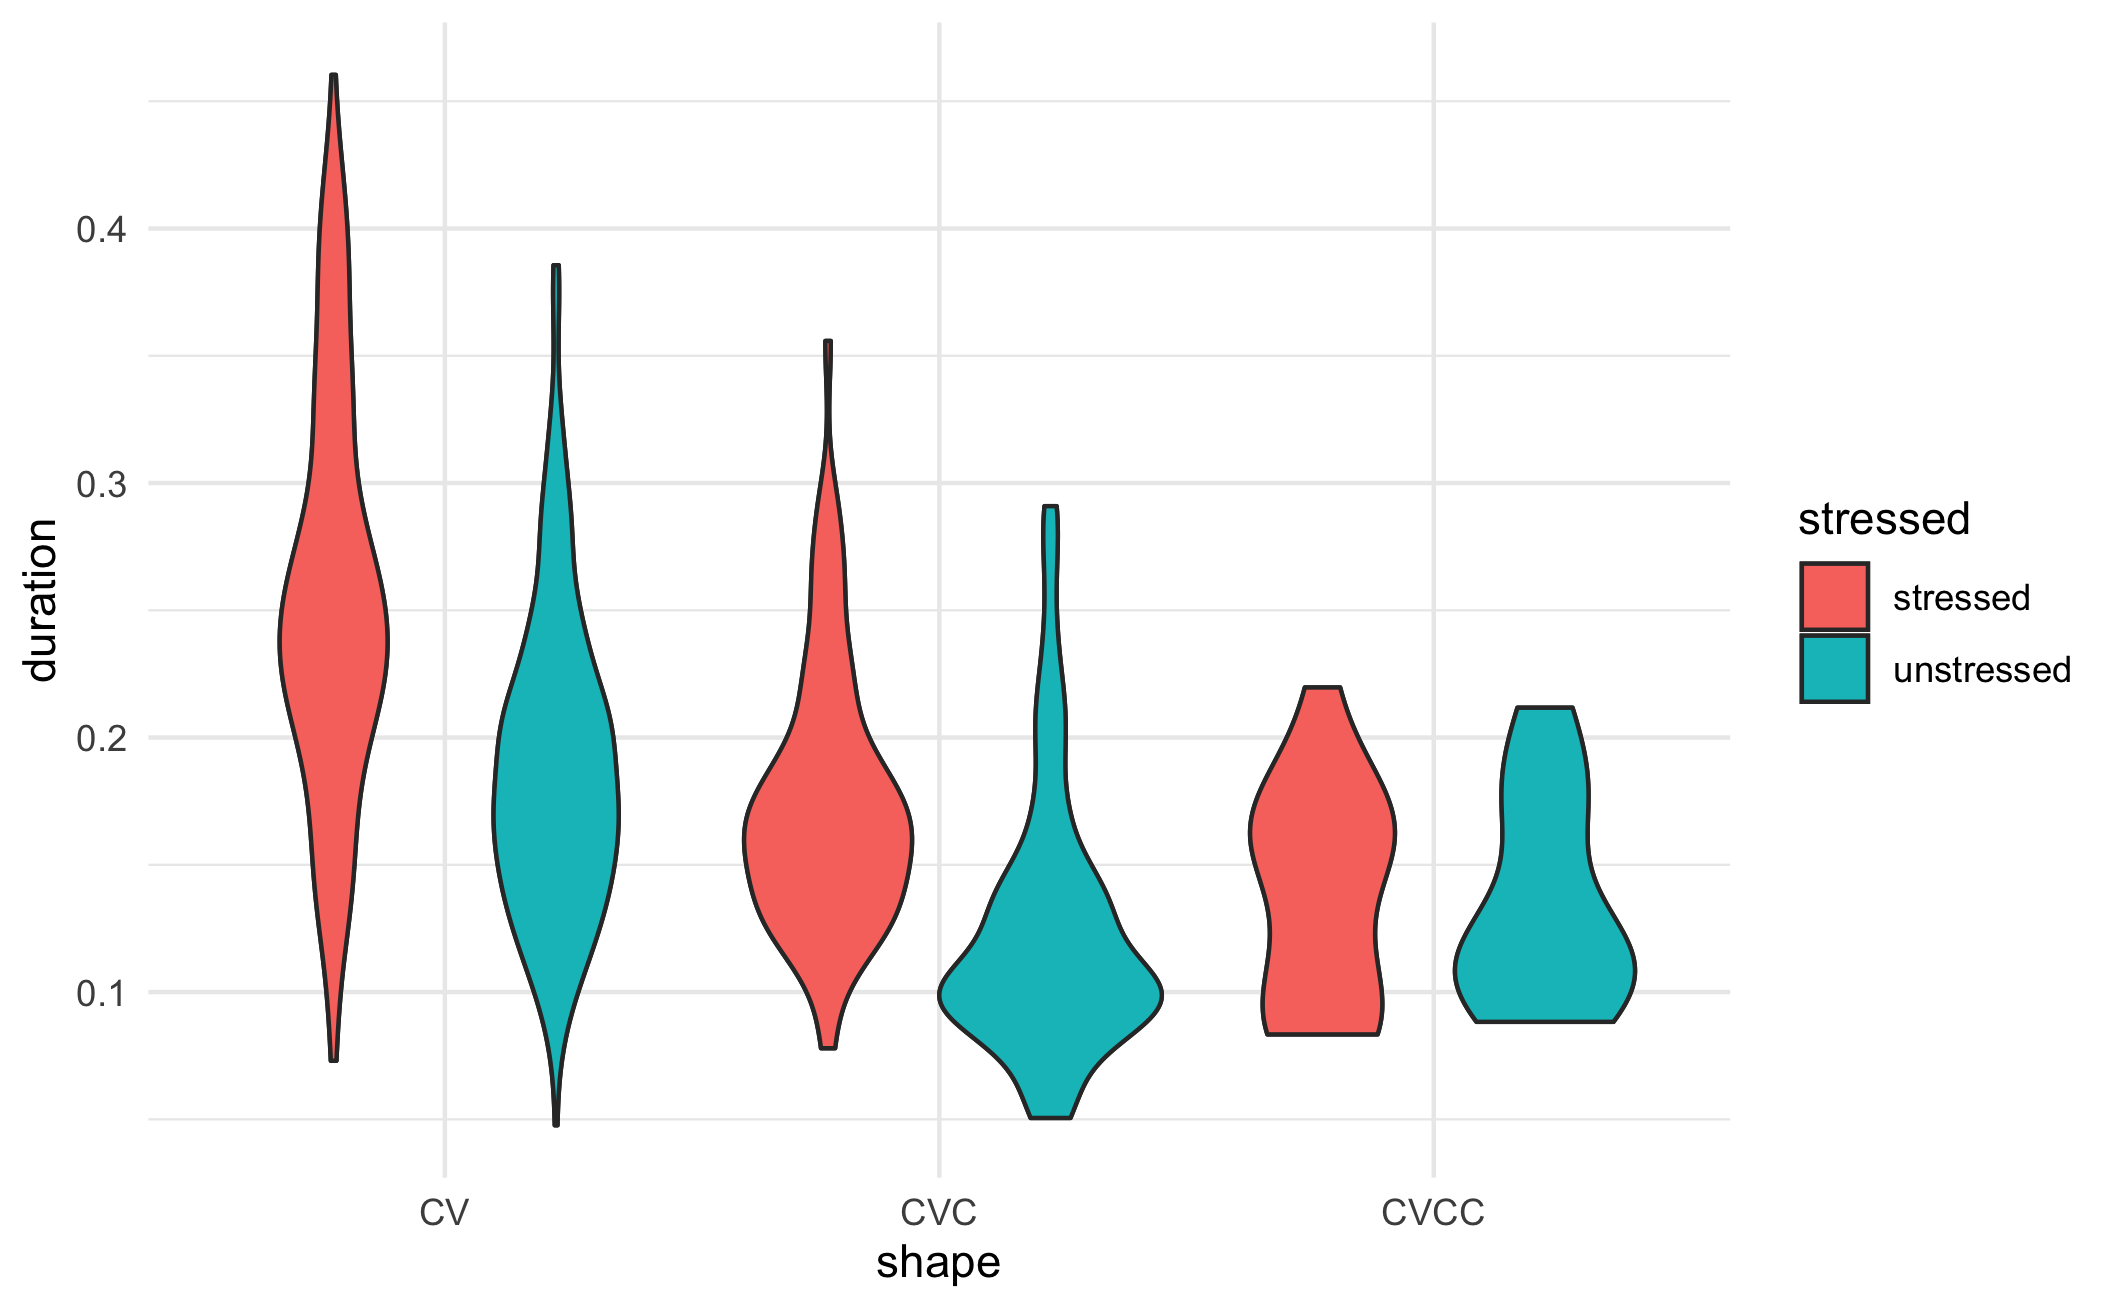
\includegraphics[width=\textwidth]{/Users/sarah/Git/regilaul_project/manuscript/results/dur_shapestress.png}
\caption{vowel dur(s) by word stress and syll. shape}
\label{strdursh}

\end{figure}
Anova comparison of the maximal design model with a null model is also statistically significant (p<0.001***). I reject the null hypothesis: these results support both word-level stress and beat position in song (ictus) as predictors for vowel duration. 

The graph in \ref{ickdursh} illustrates the distribution of vowel durations in different syllable shapes falling on and off the beat. 

A similar pattern can be seen in \ref{strdursh}, where the stressed or unstressed status is shown instead. At both song and word levels of prominence, CV or Q1 syllables are the longest, gradually decreasing in CVC and CVCC, both of which are Q2 syllables.  This further confirms the gradience of the quantity contrast at the segmental level. 



%%%%%%%%%%%%%%%%%%%%%%%%%%%%%%%%%%%%%%%%%%

%
%%%%%%%%%%%%

\subsection{Vowel Dispersion}
A subset of the Q1 and Q2 vowels used for duration measurements above is taken,  containing only those five vowel phonemes which occur in both stressed and unstressed syllables at the word level: \[a, e, i, o, u\]. The total number of vowels in this set is {\bf N}.
To account for physiological differences between singers, vowel dispersion is calculated as the euclidean distance of each token from the respective singer's vowel center in the (F1, F2) space. 


\begin{figure}[htbp]
\centering
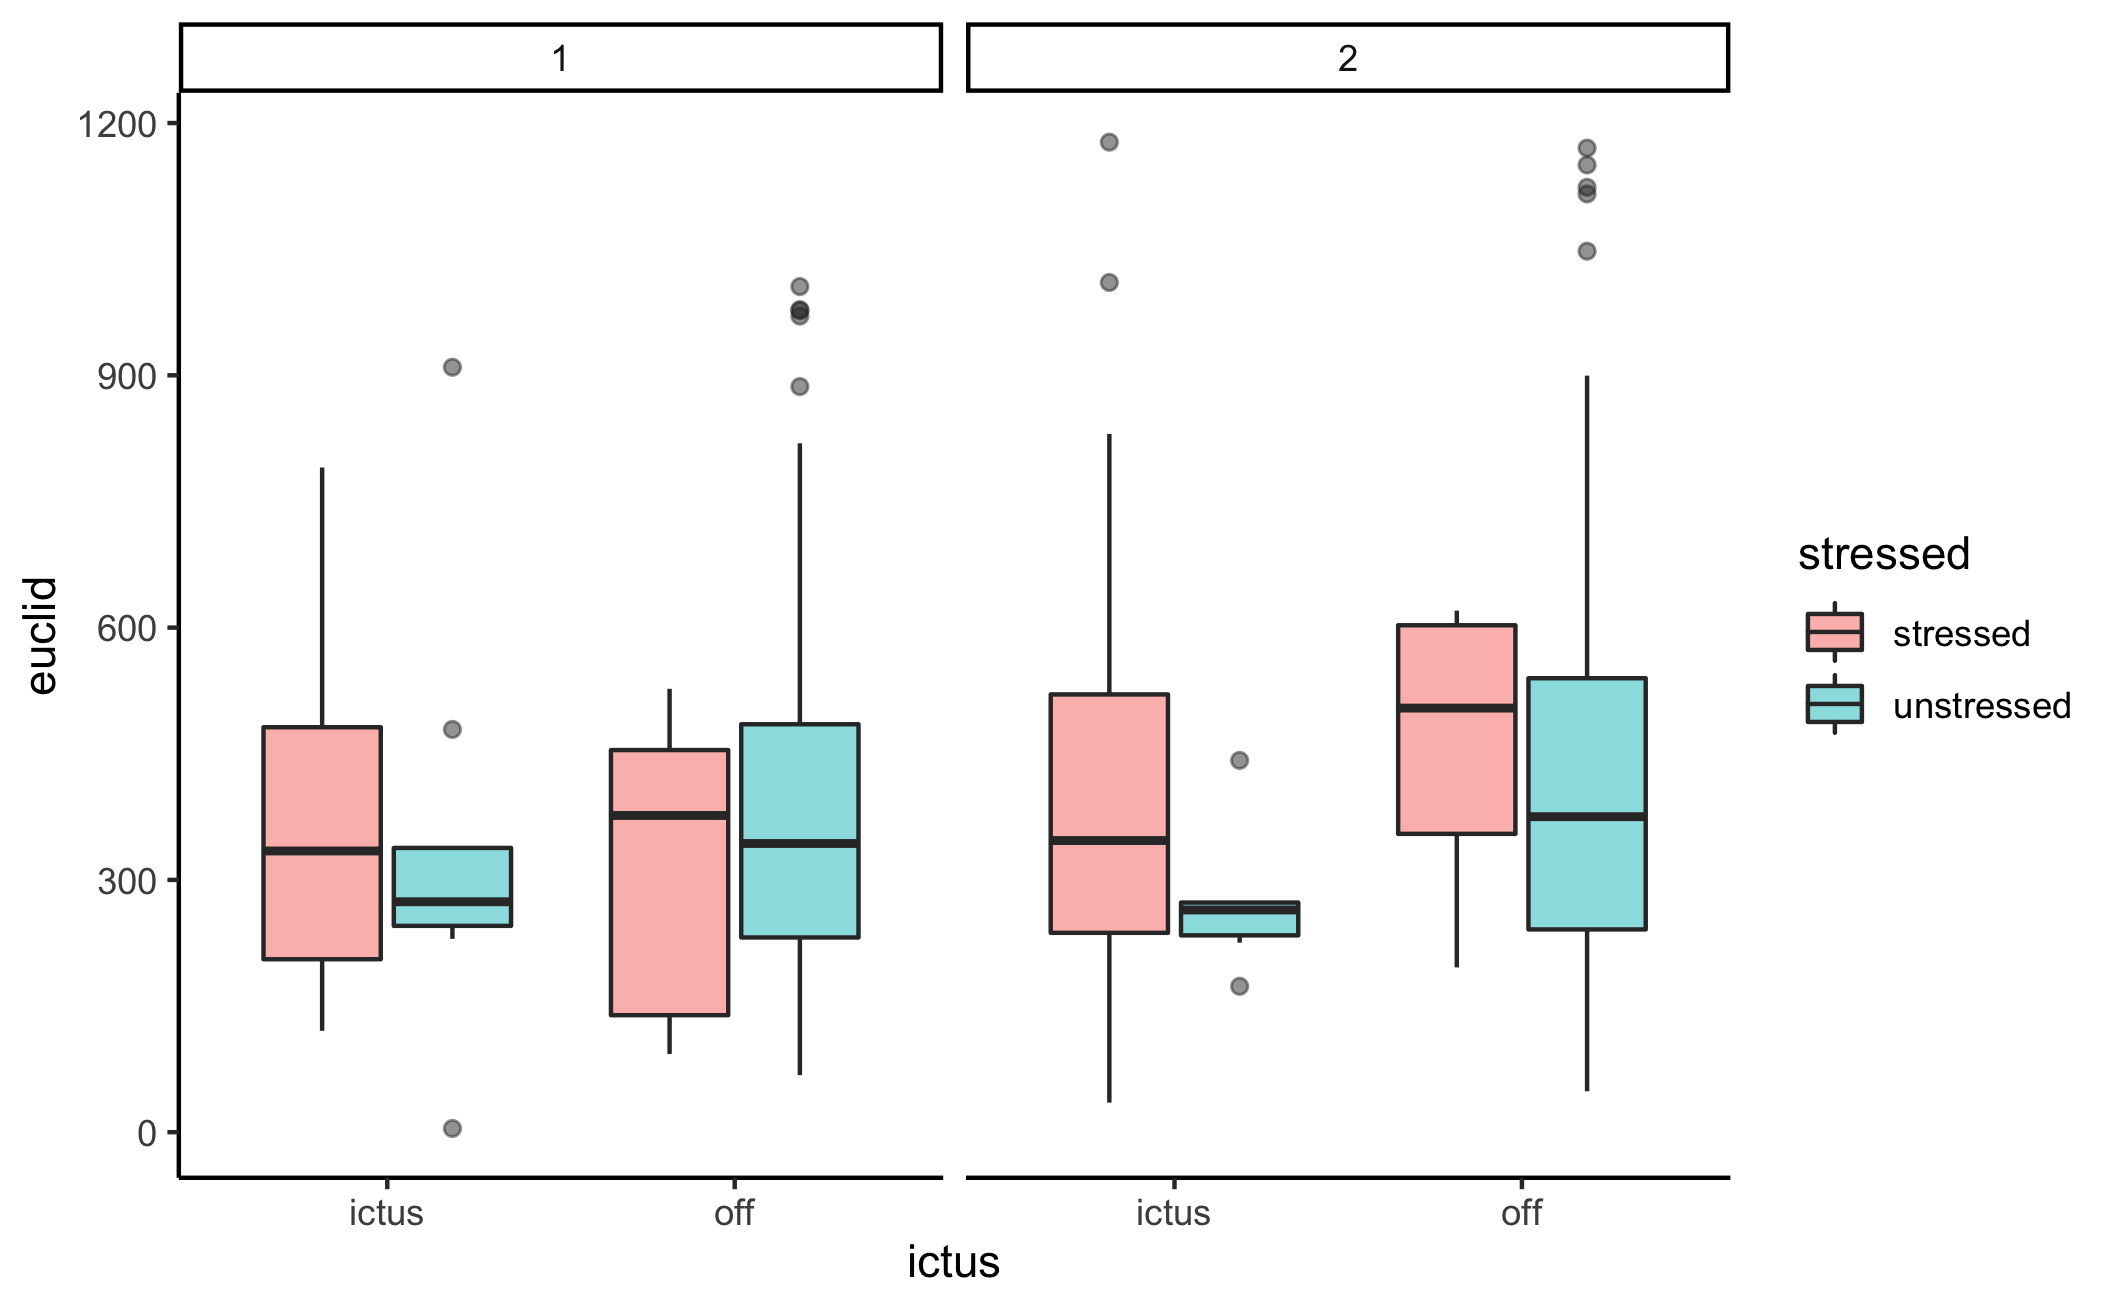
\includegraphics[width=\textwidth]{/Users/sarah/Git/regilaul_project/manuscript/results/space_strictus.png}
\caption{euclidean distance of vowels in stress and ictus}
\label{spcstrick}

\end{figure}
A pattern is marginally visible in the two graphs  \ref{spcstrick}, faceted by Q1 and Q2. Notice that in off-ictus position, vowel dispersion means of stressed syllables are higher than those of stressed syllables in ictus position. This indicates that stressed syllables falling off the beat are being compensated for their shortened vowels by way of increased articulation of quality. This pattern, however, doesn't shake out as statistically significant in the model. \\
A linear mixed effects model for vowel dispersion is constructed, but only the uninterpretable intercept shows significance. 
Comparison with null model is not statistically significant. Thus in the case of vowel dispersion, we fail to reject the null hypothesis. This could be due to the relatively smaller size of the data subset. 


